\chapter{Small oscillations}
\section{Potential energy and equilibrium}
In order to understand the general theory of oscillations, it is essential to know about the potential energl at the equilibrium configuration. Let us consider a conservative system in which the potential energy is: function of position only. Let the system be specified by $n$ generalized coordinates $q_{1}, q_{2}, \ldots, q_{n}$, not involve, time explicitly. For such a system, the potential energy is given by
$$
V=V\left(q_{1}, q_{2}, \ldots, q_{n}\right)
$$
and the generalized forces are given by
$G_{k}=-\frac{\partial V}{\partial q_{k}}$ where $k=1,2, \ldots ., n$\\
The system is said to be in equilibrium, if the generalized forces acting on the system are equal to zero: i.e.,
$$
G_{k}=-\left[\frac{\partial V}{\partial q_{k}}\right]_{0}=0
$$
\subsection{Stable,Unstable and Neutral equilibrium}
\subsubsection{Stable equilibrium}
A system is said to be in stable equilibrium, if a small displacement of the system from the rest position (by giving a little energy to it) results in a small bounded motion about the equilibrium position.
\subsubsection{Unstable equilibrium}
Small displacement of the system from the equilibrium position results in an unbounded motion, it is in an unstable equilibrium.
\subsubsection{Neutral equilibrium}
 Further, if the system on displacement has no tendency to move about or away the equilibrium position, it is said to be in neutral equilibrium.\\
 \begin{minipage}{0.5\textwidth}
 \begin{figure}[H]
 	\centering
 	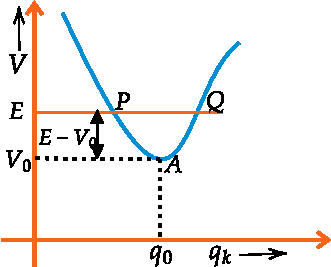
\includegraphics[height=4cm,width=5cm]{stable}
 	\caption{}
 	\label{}
 \end{figure}
 \end{minipage}
\begin{minipage}{0.5\textwidth}
\begin{figure}[H]
	\centering
	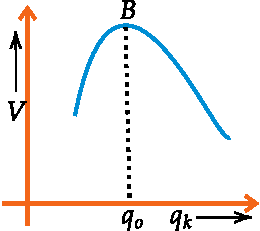
\includegraphics[height=3cm,width=5cm]{unstable}
	\caption{}
	\label{}
\end{figure}
\end{minipage}
A graph drawn between the potential energy of the system and a particular coordinate $q_{k}$ is called potential energy curve and  The positions $A$ and $B$, where the generalized force $F=-\partial V / \partial q$ vanishes, are the positions of equilibrium; potential energy $V$ is minimum (say $V_{0}$ ) at $A$ [Fig 4.1] and maximum at $B$ [Fig 4.2 ]. Position $A$ corresponds to the stable equilibrium, because if the system is displaced from $A$ to $Q$ by giving energy $\left(E-V_{0}\right)$ and left to itself, the system tries to come in the position of minimum potential energy. Consequently the potential energy will change to kinetic energy and at $A$ the energy $\left(E-V_{0}\right)$ will be purely in the kinetic form because of the conservation law. This will change again to potential form, when the system moves towards the position $P$ and hence a bounded motion ensues about the equilibrium position $A$. Obviously the position $B$ of the maximum potential energy represents the unstable equilibrium because any energy given to the system at this position will result more and more kinetic energy when the system moves either left or right to it. In this case, the system moves away from the equilibrium position. In case of neutral equilibrium, the potential energy is independent of the coordinate and equilibrium. occurs at any arbitrary value of that coordinate.
\section{Small oscillations}
In small oscillation we generalize the harmonic oscillator problem of one degree of freedom in the lagrangian formulation to the case of small amplitude oscillations of a system of seversl degrees of freedom near the position of equilibrium.When we go from a single oscillator to the problem of two coupled oscillators the analysis results in some interesting and surprising new features.We shall see that the motion of the two coupled oscillators in general is much complicated and none of the oscillators in general executes simple harmonic motion.However for small amplitude oscillations ,we may express the general motion as a superposition of two independant simple harmonic motions ,both going on simultaneously.We call thsese two simple harmonic motions as normal modes or simply modes.Further we shall see that a system of N coupled oscillators with N degrees of freedom ,has exactly N independant modes of vibration and general motion can be expressed as the superposition of N normal modes.Each mode has its own frquency and wavelength.
\subsection{Matrix method to solve small oscillations}
We shall interested in the motion of the system with in the immediate neighbourhood of configuration of stable equilibrium .Since the departure fro the equilibrium is very small ,all functions may be expanded in a Taylor series about the equlibrium ,retaining only the lowest order terms .The deviation of the generalized coordinates from equilibrium will be denoted by $\eta_i$:\\
$$q_i=q_{oi}+\eta_i$$
and these may be taken as the new generalized coordinates of the motion  
\begin{figure}[H]
	\centering
	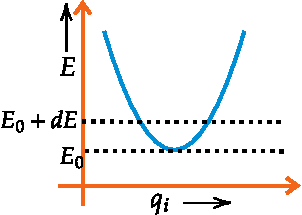
\includegraphics[height=3cm,width=5cm]{potential}
	\caption{}
	\label{}
\end{figure}
One can expand potential energy by Taylor series expansion
$$V\left(q_{i} \ldots \ldots q_{n}\right)=V\left(q_{00} \ldots \ldots q_{0 n}\right)+\left.\frac{\partial V}{\partial q_{i}}\right|_{q_{i 0}}\left(q_{i}-q_{0 i}\right)+\frac{1}{2} \frac{\partial^{2} V}{\partial q_{i} \partial q_{j}}\left(q_{i}-q_{0 i}\right)\left(q_{j}-q_{0 j}\right)+\ldots .$$
The 0 in subscript means $q_{i}=q_{0 i}$\\
So,
\begin{equation}
\quad V(q)=V_{0}+0+\frac{1}{2}\left(\frac{\partial^{2} V}{\partial q_{i} \partial q_{j}}\right)_{0} \eta_{i} \eta_{j}+\ldots \ldots \label{ref1}
\end{equation}
because at equilibrium,
$$
\left(\frac{\partial V}{\partial q_{i}}\right)_{q_{i}=q_{0 i}} \equiv\left(\frac{\partial V}{\partial q_{i}}\right)_{0}=-Q_{i}=0
$$
where $Q_{i}$ is the generalized force. Now,
\begin{equation}
V_{0} \equiv V\left(q_{01}, q_{02}, \ldots \ldots, q_{0 n}\right) \label{ref2}
\end{equation}
 is the potential energy of eqilibrium configuration whis is constant.So we set $V_0$ is equal to zero because in equations of motions only derivative of V occur.\\
 Neglecting higher order terms (because $\eta_{i}^{\prime} s$ are very small)
 \begin{equation}
 V=\frac{1}{2}\left(\frac{\partial^{2} V}{\partial q_{i} \partial q_{j}}\right)_{0} \eta_{i} \eta_{j}=\frac{1}{2} V_{i j} \eta_{i} \eta_{j} \label{ref3}
 \end{equation}
 We see that $V_{i j}=V_{j i}$
 We can write $V$ in matrix form as
\begin{align}
 V=\frac{1}{2}\left(\begin{array}{llll}
\eta_{1} & \eta_{2} & \cdots & \eta_{n}
\end{array}\right)\left[\begin{array}{cccc}
V_{11} & V_{12} & \cdots & V_{1 n} \\
V_{21} & V_{22} & \ldots & V_{2 n} \\
\vdots & \vdots & \ldots & \vdots \\
V_{n 1} & V_{n 2} & \ldots & V_{n n}
\end{array}\right]\left[\begin{array}{l}
\eta_{1} \\
\eta_{2} \\
\vdots \\
\eta_{n}
\end{array}\right]\label{ref4}
\end{align}
Since the constraints are time independent, hence kinetic energy can be written as
\begin{align}
T=\frac{1}{2} m_{i j} \dot{q}_{i} \dot{q}_{j}=\frac{1}{2} m_{i j} \dot{\eta}_{i} \dot{\eta}_{j}\label{ref5}
\end{align}
Since, $q_{i}=q_{0 i}+\eta_{i}$, so $\dot{q}_{i}=\dot{\eta}_{i}$\\
$m_{i j}$ can also be expanded similar to $V$
$$m_{i j}=m_{i j}\left(q_{01}, q_{02}, \ldots \ldots, q_{0 n}\right)+\left(\frac{\partial m_{i j}}{\partial q_{k}}\right)_{0} \dot{\eta}_{k}+\ldots \ldots \ldots$$
$\text { here we take first term only, because in equation $\ref{ref5}$ we already has } \dot{\eta} \dot{\eta}_{j} $.\\
so
\begin{equation}
T=\frac{1}{2} T_{i j} \dot{\eta}_{i} \dot{\eta}_{j}\label{ref6}
\end{equation}
$\text { where, } \quad T_{i j}=m_{i j}\left(q_{01}, q_{02}, \ldots \ldots q_{0 n}\right)$\\
\text { In matrix form, }
\begin{align}
 T=\frac{1}{2}\left(\begin{array}{llll}
\dot{\eta}_{1} & \dot{\eta}_{2} & \ldots & \dot{\eta}_{n}
\end{array}\right)\left[\begin{array}{cccc}
T_{11} & T_{12} & \ldots & T_{1 n} \\
T_{21} & T_{22} & \ldots & T_{2 n} \\
\vdots & \vdots & \ldots & \vdots \\
T_{n 1} & T_{n 2} & \ldots & T_{n n}
\end{array}\right]\left[\begin{array}{l}
\dot{\eta}_{1} \\
\dot{\eta}_{2} \\
\vdots \\
\dot{\eta}_{n}
\end{array}\right]\label{ref7}
\end{align}
Like $\mathbf{V}, \mathbf{T}$ is also symmetric, i.e. $T_{i j}=T_{j i}$
The Lagrangian is, 
\begin{align}
L=T-V=\frac{1}{2}\left(T_{i j} \dot{\eta}_{i} \dot{\eta}_{j}-V_{i j} \eta_{i} \eta_{j}\right)\label{ref8}
\end{align}
The equation of motion for $\eta_{i}$
$$
\frac{d}{d t}\left(\frac{\partial L}{\partial \dot{\eta}_{i}}\right)-\frac{\partial L}{\partial \eta_{i}}=0
$$
\begin{align}
&\frac{d}{d t}\left(\frac{\partial}{\partial \dot{\eta}_{i}}\left(T_{i j} \dot{\eta}_{i} \dot{\eta}_{j}-V_{i j} \eta_{i} \eta_{j}\right)\right)-\frac{\partial}{\partial \eta_{i}}\left(T_{i j} \dot{\eta}_{i} \dot{\eta}_{j}-V_{i j} \eta_{i} \eta_{j}\right)=0 \notag \\
&\frac{d}{d t}\left(T_{i j} \dot{\eta}_{j}\right)-V_{i j} \eta_{j}=0 \notag \\
&T_{i j} \ddot{\eta}_{j}+V_{i j} \eta_{j}=0 \label{ref9}
\end{align}
Note that $T_{i j}$ and $\mathrm{V}_{i j}$ are constants and $\dot{\eta}^{\prime} s$ and $\eta^{\prime} s$ appear only as multiplication with each other. For example the equation for $\eta_{1}$ is
\begin{align*}
&\frac{d}{d t}\left(\frac{\partial L}{\partial \dot{\eta}_{1}}\right)-\frac{\partial L}{\partial \eta_{1}}=0 \\
&\frac{d}{d t}\left[\frac{\partial}{\partial \dot{\eta}_{1}}\left(T_{1 j} \dot{\eta}_{1} \dot{\eta}_{j}\right)+\frac{\partial}{\partial \eta_{1}}\left(V_{1 j} \eta_{1} \eta_{j}\right)\right]=0
\end{align*}
[Since $V$ is independent of $\dot{\eta}^{\prime} s$ and $T$ is independent of $\eta^{\prime} s$ ]. So,
\begin{align*}
&\frac{d}{d t}\left(\frac{\partial}{\partial \dot{\eta}_{1}}\left(T_{11} \dot{\eta}_{1} \dot{\eta}_{1}+T_{12} \dot{\eta}_{1} \dot{\eta}_{2}+\ldots \ldots \ldots .+T_{1 n} \dot{\eta}_{1} \dot{\eta}_{n}+\ldots \ldots . .\right)\right)\\
&+\frac{\partial}{\partial \eta_{1}}\left(V_{11} \eta_{1} \eta_{1}+V_{12} \eta_{1} \eta_{2}+\ldots \ldots . . V_{1 n} \eta_{1} \eta_{n}+\ldots \ldots\right)=0 \\
&\frac{d}{d t}\left(T_{11} \dot{\eta}_{1}+T_{12} \dot{\eta}_{2}+\ldots \ldots T_{1 n} \dot{\eta}_{n}\right)+\left(V_{11} \eta_{1}+V_{12} \eta_{2}+\ldots \ldots+V_{1 n} \eta_{n}\right)=0 \\
&T_{11} \ddot{\eta}_{1}+T_{12} \ddot{\eta}_{2}+\ldots . .+T_{1 n} \ddot{\eta}_{n}+\left(V_{11} \eta_{1}+V_{12} \eta_{2}+\ldots . .+V_{1 n} \eta_{n}\right)=0
\end{align*}
In summation convention the above equation is
\begin{align}
T_{1 j} \ddot{\eta}_{j}+V_{1 j} \eta_{j}=0\label{ref10}
\end{align}
The point is that you should know what any expression means. So, we get $\eta$ equations in total.
To sovle the equation of motion $\eta$, we put a trial solution.

\begin{equation}
\eta_{j}=C a_{j} e^{-i o t}\label{ref11}
\end{equation}
Note that in the exponential $i=\sqrt{-1}$
We get,
\begin{align}
&\dot{\eta}_{j}=-C a_{j}(i \omega) e^{-i \omega t} \notag \\
&\ddot{\eta}_{j}=+C a_{j}(i \omega)^{2} e^{-i \omega t}=-\omega^{2} \eta_{j}\label{ref12}
\end{align}
$\text { putting } \ddot{\eta}_{j} \text { in equation ($\ref{ref9}$) }$
\begin{align}
&T_{i j} \ddot{\eta}_{j}+V_{i j} \eta_{j}=0 \notag\\
&T_{i j}\left(-\omega^{2} \eta_{j}\right)+V_{i j} \eta_{j}=0 \notag\\
&\left(V_{i j}-\omega^{2} T_{i j}\right) \eta_{j}=0\label{ref13} \\
&V_{i j} a_{j}=\omega^{2} T_{i j} a_{j}\label{ref14}
\end{align}
 in the matrix form equation ($\ref{ref13}$), is (equation  $\ref{ref14}$  also can be written in similar form)\\
 $\left[\begin{array}{cccc}
 	V_{11} & V_{12} & \ldots & V_{1 n} \\
 	V_{21} & V_{22} & \ldots & V_{2 n} \\
 	\vdots & \vdots & & \vdots \\
 	V_{n 1} & V_{n 2} & \ldots & V_{n n}
 \end{array}\right]\left[\begin{array}{l}
 	\eta_{1} \\
 	\eta_{2} \\
 	\vdots \\
 	\eta_{n}
 \end{array}\right]-\omega^{2}\left[\begin{array}{cccc}
 	T_{11} & T_{12} & \ldots & T_{1 n} \\
 	T_{21} & T_{22} & \ldots & T_{2 n} \\
 	\vdots & \vdots & & \vdots \\
 	T_{n 1} & T_{n 2} & \ldots & T_{n n}
 \end{array}\right]\left[\begin{array}{l}
 	\eta_{1} \\
 	\eta_{2} \\
 	\vdots \\
 	\eta_{n}
 \end{array}\right]=0$
 \begin{align}
 \left[\begin{array}{cccc}
 V_{11}-\omega^{2} T_{11} & V_{12}-\omega^{2} T_{12} & \ldots & V_{1 n}-\omega^{2} T_{1 n} \\
 V_{21}-\omega^{2} T_{21} & V_{22}-\omega_{2} T_{22} & \ldots & V_{2 n}-\omega^{2} T_{2 n} \\
 \vdots & \vdots & & \vdots \\
 V_{n 1}-\omega^{2} T_{n 1} & V_{n 2}-\omega^{2} T_{n 2} & & V_{n n}-\omega^{2} T_{n n}
 \end{array}\right]\left[\begin{array}{l}
 \eta_{1} \\
 \eta_{2} \\
 \vdots \\
 \eta_{n}
 \end{array}\right]=0\label{ref15}
 \end{align}
 From properties of matrices we know that for equation ($\ref{ref15}$) to be satisfied for all $\eta^{\prime} s$. The determinant of matrix $\mathbf{V}-\omega^{2} \mathbf{T}$ must be zero i.e.
 $$
 \left|\mathbf{V}-\omega^{2} \mathbf{T}\right|=0
 $$
 \begin{align}
 \left|\begin{array}{cccc}
 V_{11}-\omega^{2} T_{11} & V_{12}-\omega^{2} T_{12} & \cdots & V_{1 n}-\omega^{2} T_{1 n} \\
 V_{21}-\omega^{2} T_{21} & V_{22}-\omega_{2} T_{22} & \cdots & V_{2 n}-\omega^{2} T_{2 n} \\
 \vdots & \vdots & & \vdots \\
 V_{n 1}-\omega^{2} T_{n 1} & V_{n 2}-\omega^{2} T_{n 2} & & V_{n n}-\omega^{2} T_{n n}
 \end{array}\right|=0\label{ref16}
 \end{align}
  This equation ($\ref*{ref16}$) is called the secular equation.
  By solving the determinant ($\ref{ref16}$) we get $n$ values of $\omega^{2}$. Each value of $\omega$ represents the frequency of normal mode. The equation ($\ref{ref14}$) is a type of eigenvalues. $\mathbf{V}$ acting on eigenvector a gives $\omega^{2} \mathbf{T a}$. There are $n$ such eigenvectors. Hence, there are $n$ normal modes. It can be shown that the eigen vector matrix of which is denoted by $\mathbf{A}$ diagonalizes both $\mathbf{T}$ and $\mathbf{V}$ (for detail see section $6.2$ of Goldstein, $3^{\text {rd }}$ eddition, but it is sufficient for us to rememher the result). A diagonalizes $\mathbf{V}$ to a matrix whose diagonal elements are the eigen-$\text { values i.e. } \omega^{2 \prime} s \text { (say } \lambda^{\prime} s)$\\
  (Note that in ordinary eigen alue problems, matrix acting on eigenvector produces eigenvalue times the eigenvector i.e. $\mathbf{M a}=\lambda \mathbf{a}$ or $(\mathbf{M}-\lambda \mathbf{1}) \mathbf{a}=0$, but here it is $(\mathbf{V}-\lambda \mathbf{T}) \mathbf{a}=0 .)$\\
  ie
  \begin{align}
  \tilde{\mathbf{A}} \mathbf{V} \mathbf{A}=\lambda=\left[\begin{array}{cccc}
  \lambda_{1} & 0 & \cdots & 0 \\
  0 & \lambda_{2} & \cdots & 0 \\
  \vdots & \vdots & & \vdots \\
  0 & 1, & \cdots & \lambda_{n}
  \end{array}\right]\label{ref17}
  \end{align}
  $\text { where } \lambda_{1}, \lambda_{2} \ldots . . \text { are eigen values of (i.e. } \omega^{21} s \text { ) }$\\
  And $\mathbf{T}$ is diagonalized to identity i.e.
  \begin{align}
  \tilde{\mathbf{A}} \mathbf{T} \mathbf{A}=\mathbf{1}\label{ref18}
  \end{align}
  To solve a problem, the main thing we need to do is\\
   (1) Solve the determinant (9.16) to find the frequencies of normal modes\\
  (2) Find the eigenvectors a correspoinding to each $\omega^{2}$ (the eigenvalue), in the equation.
  $$
  \left(\mathbf{V}-\omega^{2} \mathbf{T}\right) \mathbf{a}=0
  $$
  where the $k^{\text {th }}$ eigenvector (corrersponding to $k^{\text {th }} \omega^{2}$ )
  
  \begin{align}
  \mathbf{a}_{k}=\left[\begin{array}{c}
  a_{1 k} \\
  a_{2 k} \\
  \vdots \\
  a_{n k}
  \end{array}\right]\label{ref19}
  \end{align}
  (3) The normal mode coordinates are
  \begin{align}
  Q_{k}=f_{k} \cos \left(\omega_{k} t+\delta_{k}\right)\label{ref20}
  \end{align}
  where, $f_{k}$ and $\delta_{k}$ are amplitude and phase factor respectively. Note that in a normal mode, the hole system oscillates with same frequency.
  (4) The general solution for
  \begin{align}
  \eta_{i}=a_{i k} Q_{k}\label{ref21}
  \end{align}
   The matrix $\mathbf{A}$ is 
   \begin{align}
   \left[\begin{array}{llll}a_{11} & a_{12} & \cdots & a_{1 n} \\ a_{21} & a_{22} & \cdots & a_{2 n} \\ \vdots & \vdots & & \vdots \\ a_{n 1} & a_{n 2} & \cdots & a_{n n}\end{array}\right]\label{22}
   \end{align}
  So, the solution of our problem (the equation ($\ref{ref21}$) is:
 \begin{align}
  \left[\begin{array}{l}
 \eta_{1} \\
 \eta_{2} \\
 \vdots \\
 \eta_{n}
 \end{array}\right]=\left[\begin{array}{llll}
 a_{11} & a_{12} & \cdots & a_{1 n} \\
 a_{21} & a_{22} & \cdots & a_{2 n} \\
 \vdots & \vdots & & \vdots \\
 a_{n 1} & a_{n 2} & \cdots & a_{n n}
 \end{array}\right]\left[\begin{array}{l}
 Q_{1} \\
 Q_{2} \\
 \vdots \\
 Q_{n}
 \end{array}\right] 
 \end{align}
 One complication may arise when eigenvalues are degenerate. In this case we first choose an eigenvector (corresponding to degenerate eigenvalue) satisfying the eigenvalue equation and remaining eigenvectors (if there is $k$-fold degeneracy, then there are $k$-eigenvectors corresponding to single eigenvalue) are determined such that they satisfy the eigenvalue equation and are orthogonal to each other.